\documentclass{article}
\usepackage[a4paper, left = 25mm, right = 25mm, bottom = 25mm]{geometry}
\usepackage{amsmath}
\usepackage{graphicx}
\usepackage{float}
\usepackage{hyperref}
\usepackage{fancyvrb}
\usepackage{matlab-prettifier}
\usepackage{enumitem}
\usepackage{color}
% \usepackage{minted}
\usepackage{palatino}
\usepackage{listings}
\usepackage{xcolor}
\usepackage{tcolorbox}  % For rounded boxes
\usepackage{courier}    % For custom font style
\fontfamily{SansSerif}

\setlength{\parindent}{0pt}

\title{EE324: Control Systems Lab \\ Experiment 4: Noise Cancellation in Headphones\\ \textbf{Group 1 - Thursday}}
\author{\large Harsh S Roniyar\\ \large 22B3942 \and \large Pranav Prakash\\ \large 22B3945 \and \large Aman Verma\\ \large 22B3929}

\begin{document}

\maketitle

\section{Objective}

Design and implement an analog circuit for noise cancellation in headphones.
\vspace{5pt}

The specific objectives were:
\begin{itemize}[noitemsep]
  \item To achieve an attenuation of 20 dB (not necessarily exact 20, small attenuation also works if the system is stable) when a noise of 100 Hz frequency is applied.
  \item To design an analog compensator to stabilize the system, i.e., loop shaping of the loop transfer function.
\end{itemize}

\section{Control Algorithm}

For the given headphone- microphone setup, we had to characterize by finding out the transfer characteristics of the headphone setup. Let us call it G(s). 

The closed loop can be modelled as a unity feed-back model. We were required to add a controller C(s) in the feedforward path to ensure that the given characteristics are met. The transfer function of the closed-loop system is given by:
\[ \frac{Y(s)}{X(s)} = \frac{1}{1 + C(s)G(s)} \]

\section{Methodology}

We initially examined the headphone setup to understand its open-loop output transfer characteristics. Subsequently, we employed \texttt{MATLAB} tools to model the compensated stable system using a second-order approximation based on the gathered data. Following this, our attention turned to identifying suitable values of resistances and capacitors in the compensator, labeled as \(C(s)\).

The specific aim was to choose such a compensator that, at a frequency of 100 Hz, achieves a 20 dB (or similar) attenuation in the output-to-noise transfer function while also remaining stable. It's crucial to emphasize that this analysis is centered on noise cancellation headphones, with a primary emphasis on enhancing the system's efficiency in minimizing undesired noise.

\subsection{Procedure}

Frequency response analysis is performed on the headphone setup with sinusoidal waves given as input, from the function generator. Both the input and output are observed in the DSO, and then the magnitude and phase bode plots are plotted versus frequency. This is the open-loop characteristic of headphones.

\subsubsection{Compensator Design}

The compensator is designed to stabilize the system and achieve the desired attenuation at 100 Hz. The compensator is a second-order system, and the parameters are chosen to meet the requirements.

The circuit diagram for the compensator is shown below:
\begin{figure}[!htb]
    \centering
    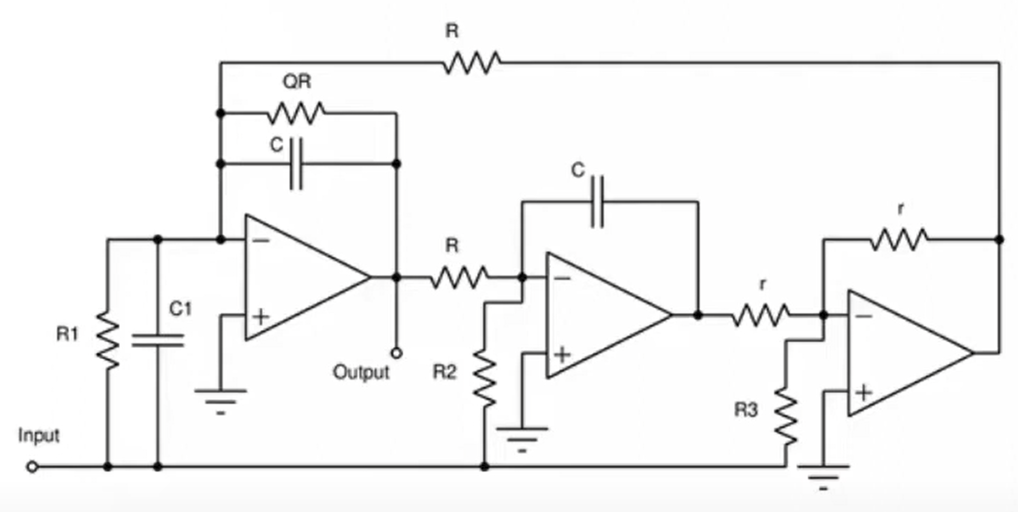
\includegraphics[width=0.5\textwidth]{image.png}
    \caption{Second Order Compensator Circuit Diagram}
    \label{fig:compensator}
\end{figure}

The transfer function of the compensator is given by:
\[ C(s) = \frac{as^2 + bs + c}{ds^2 + es + f} \]
which in terms of the circuit components is:
$$ C(s) = \frac{\left(\frac{C_1}{C}\right)^2 s^2 + \frac{1}{C}\left(\frac{1}{R_1} - \frac{r}{R\cdot R_3}\right)s + \frac{1}{C^2\cdot R\cdot R_2}}{s^2 + \frac{1}{Q\cdot C\cdot R}s + \frac{1}{C^2\cdot R^2}} $$

The values of the parameters are chosen such that the compensator meets the requirements. The bode plot of the compensator is plotted in MATLAB to verify the design.

\begin{figure}
    \centering
    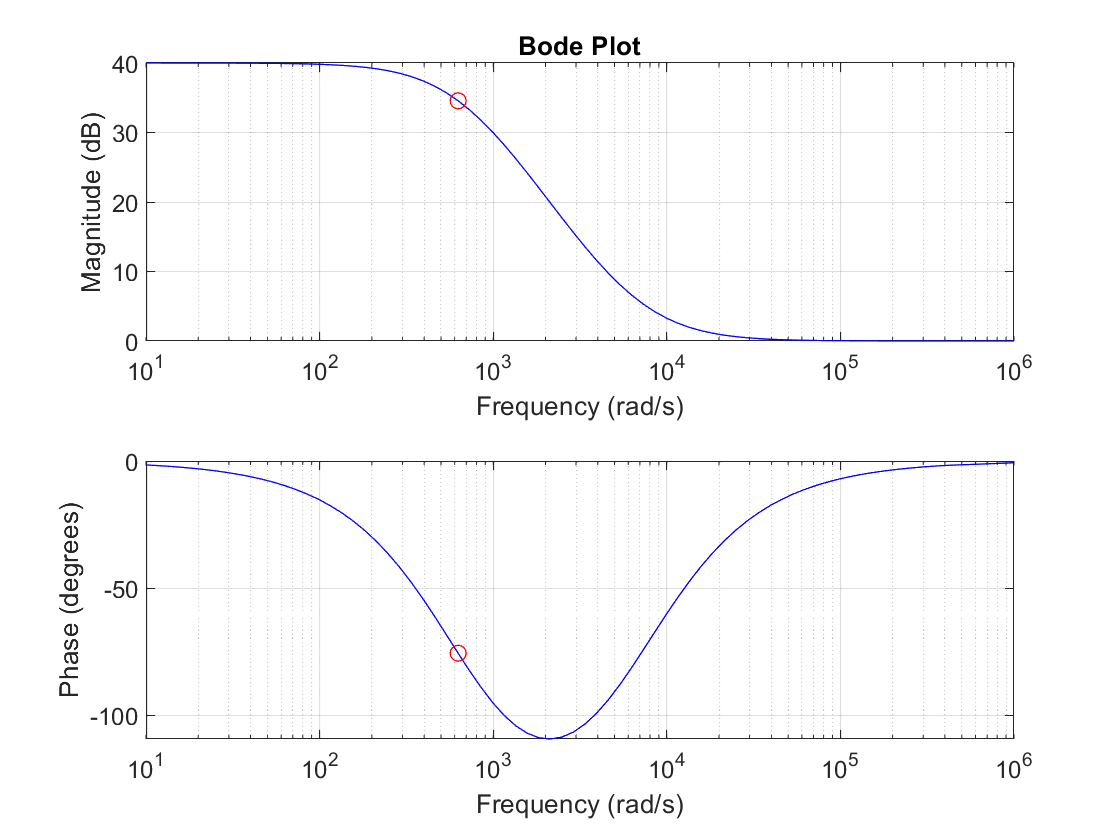
\includegraphics[width=0.75\textwidth]{bode-plot.png}
    \caption{Bode Plot of the Compensator}
    \label{fig:bode}
\end{figure}

The values of the circuit components chosen are as follows:

\begin{table}[!htb]
  \centering
  \begin{tabular}{|c|c|}
    \hline
    Parameter & Value \\ \hline
    \( C_1 \) & 150 pF \\ 
    \( C \) & 150 pF \\ 
    \( R_1 \) & 330 k\(\Omega\) \\ 
    \( R \) & 10 M\(\Omega\) \\ 
    \( R_3 \) & 100 \(\Omega\) \\ 
    \( R_2 \) & 100 k\(\Omega\) \\ 
    \( Q \) & 0.5 \\ 
    \( r \) & 1 k\(\Omega\) \\ \hline
  \end{tabular}
  \caption{Circuit Component Values}
\end{table}

\newpage
\section{Challenges Faced and Solutions}
\begin{enumerate}[left=0pt, label=\textbf{Problem \arabic*}:, itemsep=10pt]
  \item \textbf{Noisy Readings:} We initially obtained noisy readings in our characterization of the headphone setup due to ambient disturbances in the surroundings. \\
  \underline{\textit{Solution:}} We repeated the experiment in a different, quieter environment, which allowed us to obtain observational readings suitable for controller design.

  \item \textbf{MATLAB Bode Plot:} When plotting the Bode plot in MATLAB, we were unaware that the input parameters for the \texttt{bode()} function are given in radians rather than Hertz, which led to incorrect results. \\
  \underline{\textit{Solution:}} We corrected this by converting the frequency units from Hertz to radians before plotting, resolving the discrepancy.

  \item \textbf{Optimum Resistance and Capacitance Values:} The exact values of resistances and capacitances were unavailable, necessitating approximations. \\
  \underline{\textit{Solution:}} We matched the resistance and capacitance values as closely as possible to achieve a functional circuit implementation.
\end{enumerate}

\section{Results}

The compensator was successfully designed to achieve targeted noise attenuation and improve the stability of the system. The following key results were observed:

\begin{itemize}%[noitemsep]
    \item The designed compensator transfer function is $$C(s) = \frac{(s+6500)^2}{(s+650)^2}$$
    \item \textbf{Gain Margin (Before Compensation at 100 Hz):} The gain margin of the open-loop system at 100 Hz before compensation was measured at \( 5.69 \) dB.
    \item \textbf{Phase Margin (Before Compensation at 100 Hz):} The phase margin at 100 Hz before compensation was measured at \( \infty \) degrees.
    \item \textbf{Gain Margin (After Compensation at 100 Hz):} The gain margin at 100 Hz after adding the compensator was measured at \( 3.32 \) dB, indicating stability.
    \item \textbf{Phase Margin (After Compensation at 100 Hz):} The phase margin at 100 Hz after compensation increased to \( 49.2 \) degrees, further contributing to the system's stability.
    \item \textbf{Gain at 100 Hz (Before Compensation):} The gain at 100 Hz in the open-loop configuration, before adding the compensator, was \( -6.67 \) dB.
    \item \textbf{Gain at 100 Hz (After Compensation):} After incorporating the compensator, the open-loop gain at 100 Hz was \( 7.43 \).
\end{itemize}

The Bode plots of both the open-loop compensated system and the closed-loop compensated system are shown below. These plots illustrate the frequency response characteristics, showing the effects of compensation on the system's stability and noise attenuation performance:

\begin{figure}[!htb]
    \centering
    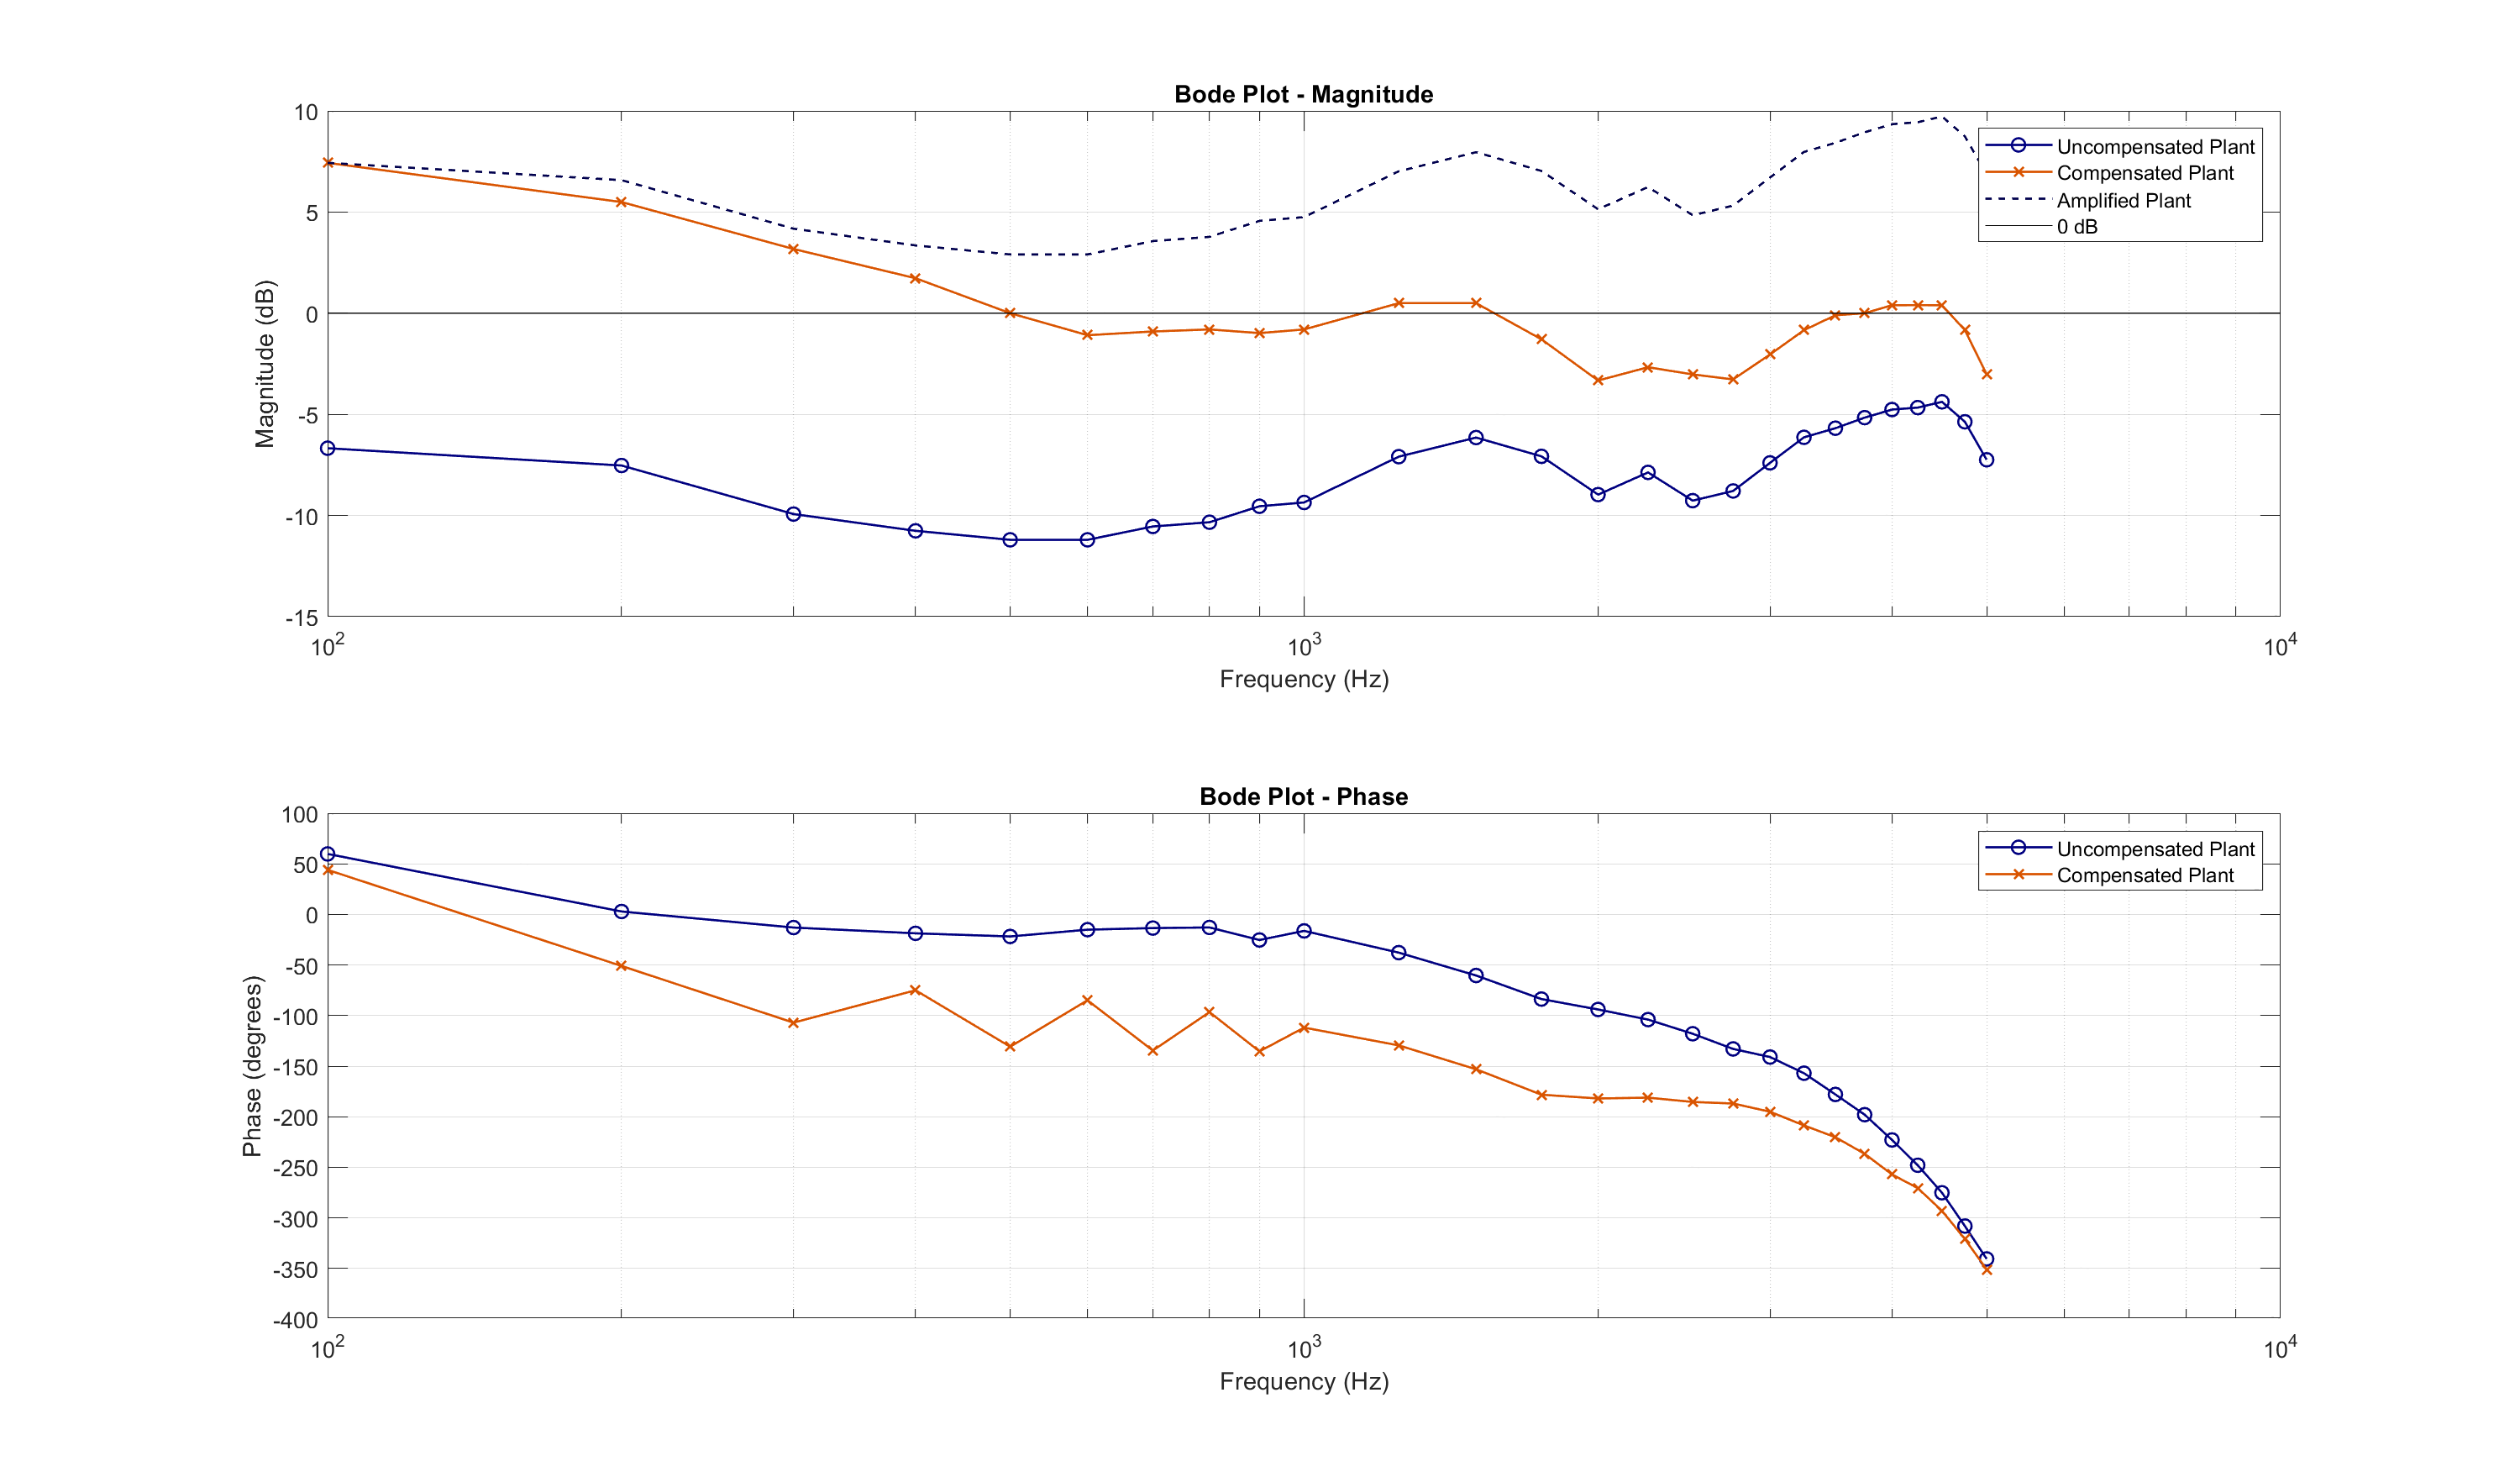
\includegraphics[width=\textwidth]{open_loop_2.png}
    \caption{Bode Plot of the Open-Loop Compensated System}
    \label{fig:bode_open_loop}
\end{figure}

\begin{figure}[!htb]
    \centering
    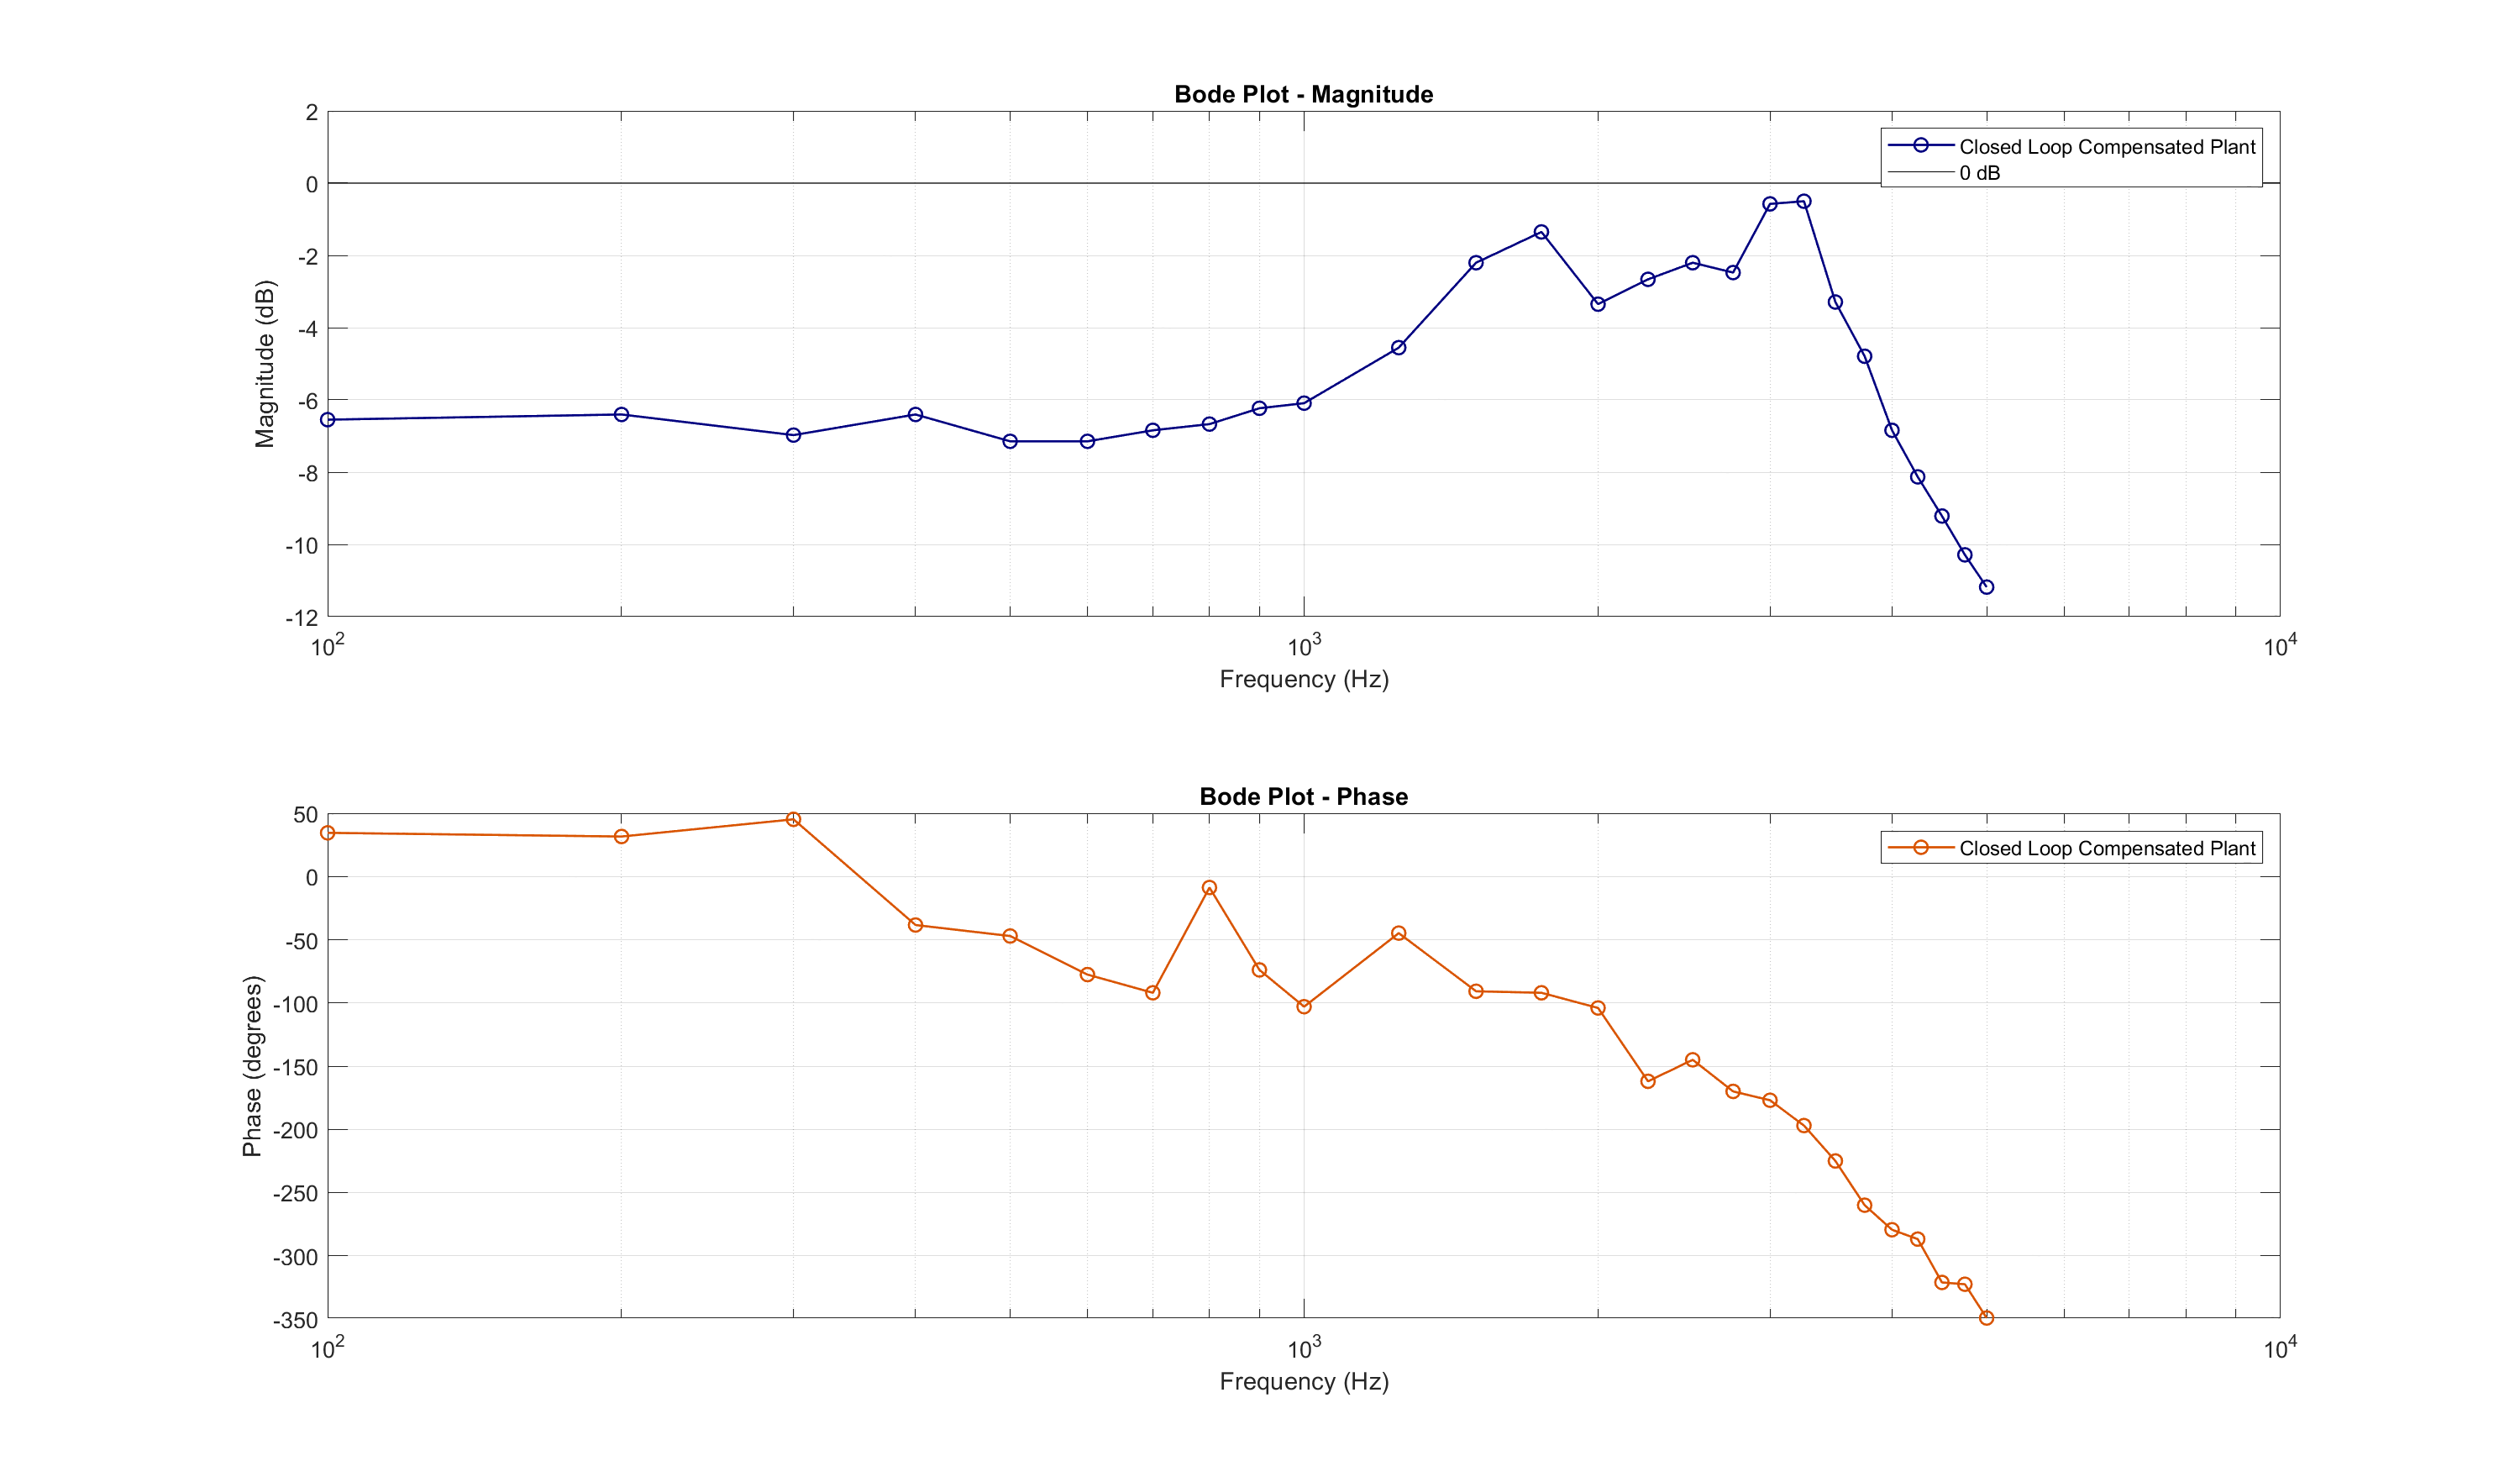
\includegraphics[width=\textwidth]{closed_loop_2.png}
    \caption{Bode Plot of the Closed-Loop Compensated System}
    \label{fig:bode_closed_loop}
\end{figure}

\newpage
\section{Observations and Inference}

\begin{itemize}%[noitemsep]
    \item The compensator successfully achieved an attenuation at 100 Hz, which effectively reduced noise interference.
    \item The reduction in gain at 100 Hz from \( 7.43 \) dB to approximately \( -7 \) dB after closed-loop compensation indicates successful attenuation, meeting the noise reduction objectives.
    \item The Bode plots demonstrate that the compensator adequately shapes the loop transfer function, which is evident from the smoother transition in gain and phase, thus stabilizing the system and ensuring efficient noise cancellation.
    \item This success in noise cancellation for headphones highlights the potential for similar compensator designs in various analog noise reduction applications.
\end{itemize}

\end{document}
